\documentclass[a4paper, 12pt]{article}
\usepackage{geometry}
\geometry{margin=2cm}
\usepackage{graphicx} % Required for the inclusion of images
\usepackage[utf8]{inputenc}
%\usepackage{natbib} % Required to change bibliography style to APA
\usepackage{amsmath} % Required for some math elements 
\usepackage[spanish]{babel} 
%\usepackage{fontspec}
\usepackage{lineno,hyperref}
\usepackage{upgreek}
\usepackage{gensymb}
\usepackage{textcomp}
\usepackage{amssymb}
\usepackage{textgreek}
\usepackage{float}
\usepackage{fancyhdr}
\usepackage{dirtytalk}

\allowdisplaybreaks
%\textwidth18cm
%\textheight22cm
%\topmargin0cm
%\oddsidemargin2cm
%\hypersetup{hidelinks}

\usepackage{multirow}

\hypersetup{
    colorlinks=true,
    linkcolor=blue,
    }
\graphicspath{{img}}
\setlength\parindent{0pt} % Removes all indentation from paragraphs

\renewcommand{\labelenumi}{\alph{enumi}.} % Make numbering in the enumerate environment by letter rather than number (e.g. section 6)

\renewcommand{\b}{\bf}

\newsavebox{\mygraphic}
\sbox{\mygraphic}{
\includegraphics[height=1cm]{logoUNRN.jpg}}


\pagestyle{fancy}

\fancyhead{}

\headheight 16pt

\fancyhead[LO]{\setlength{\unitlength}{1in}
	\begin{picture}(0,0)
		\put(0,0){\usebox{\mygraphic}}
	\end{picture}
	\hspace{1cm}
}

\fancyhead[CO] {\hspace{1.5cm} \large Física I: Ingenierías Ambiental, Electrónica y Telecomunicaciones}

%esto me pareció piola para enumerar los ejercicios
%lo saqué de acá: https://tex.stackexchange.com/questions/302948/numbered-exercises-as-sections
%%%%%%%%%%%%%%%%%%%%%%%%%%%%%%%%%%%%%%%%%5
\newcounter{eje}
\setcounter{eje}{0}
\newcounter{subeje}
\setcounter{subeje}{-1}
\renewcommand\thesubeje{\arabic{eje}\alph{subeje}}%
\newcommand \eje{%
  \vspace{.2cm}
  \par\noindent
  \ifnum\value{subeje}>-1
    \refstepcounter{subeje}%
    \llap{\thesubeje)\quad}%
  \else
    \refstepcounter{eje}%
    \llap{\theeje)\quad}%
  \fi
}
\begin{document}
\pagestyle{fancy}

\begin{center}

	{\Large \bf{Final Física I (Diciembre 2023)}}
 
\vspace{.2cm}

{miércoles 6/12}
\end{center}

%\hspace{5cm}Tome para el valor de g = 9.8 m/s$^2$.
\begin{itemize}
	\item Resuelva cada ejercicio en una hoja separada
	\item Si las cantidades que se piden son dimensionales, acompañe el valor con la unidad correspondiente
	\item De las respuestas con precisión numérica consecuente con los datos
	\item para la gravedad utilice g = 9.8 m/s$^2$.
\end{itemize}

\eje Un carrito de masa M = $0.25$ kg, inicialmente en reposo, se deja caer por un plano inclinado para luego tomar una rampa que lo deja en caída libre al ras del suelo, forzando una dirección de 30$\degree$ en la velocidad inicial. Luego del vuelo libre el carrito vuelve a tocar el suelo a una distancia $d = 1$m., Si el carrito se soltó desde una altura $h = 1.5$m
\begin{itemize}
  \item[a)] Determine el trabajo de las fuerzas no conservativas (sin omitir el signo ya sea positivo o negativo)
  %rta Wnc = Ef - Ei = K - Upot = 1/2 M g d/sen(60) - Mgh = -0.35m Mg = -0.846 J
  
  \item[b)] Suponiendo que las fuerzas no conservativas actúan únicamente a lo largo de 2 metros del plano inclinado, ¿cuál será el coeficiente de roce dinámico $\mu_d$? Realice un diagrama de cuerpo libre si fuera necesario.
% rta: Wnc = -1* Mgcos(37) * \mu * 2 m = -0.35 Mg  --> \mu =0.35/2/0.8 = .22
  
  \item[c)] ¿Qué fracción de la energía potencial inicial se disipa por el trabajo de las fuerzas de roce? (Considere el cero a nivel del suelo)
  
%  rta:   Upot * q = |Wnc|
%         Mg 1.5m q = 0.35m Mg --> q = 0.23

  \item[d] ¿Cuál es el módulo de la velocidad al inicio del vuelo libre?  
  %acá está la clave del problema
  %rta v0 = \sqrt{g d /sen(2\theta)} = 3.37 m/s
\end{itemize}
\begin{figure}[H]
\begin{center}
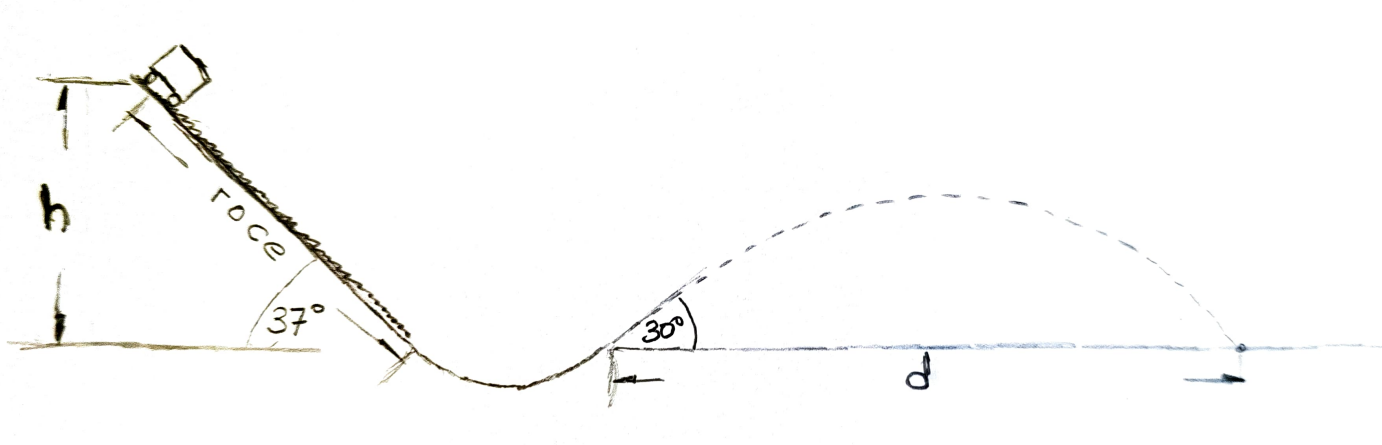
\includegraphics[clip,width = \columnwidth]{img/ener-roce_final_dic2023.png}
\end{center}
\end{figure}

\end{document}